% begin module natural-logarithm-def-ex8
\begin{frame}
\begin{example}%[Example 8, p. 408]
Draw the graph of $y = \ln (x - 2) -1$.
\begin{columns}[c]
\column{.55\textwidth}
\psset{xunit=1cm, yunit=1cm}
\begin{pspicture}(-0.5,-3)(6,2.5)
\psframe*[linecolor=white](-0.5,-3)(6,2.5)
\psaxes[ticks=none, labels=none]{<->}(0,0)(-0.5,-3)(6,2.5)
\fcLabelXOne
\fcLabelYOne
\uncover<2>{
\psplot[linecolor=red, plotpoints=1000]{0.049787068}{6}{x ln}
\rput[lb](0.6, 0.8){\footnotesize $y=\ln(x)$}
}
\uncover<3->{
\psplot[linecolor=gray, plotpoints=1000]{0.049787068}{6}{x ln}
\rput[lb](0.6, 0.8){\color{gray}\footnotesize $y=\ln(x)$}
}
\uncover<3>{
\psplot[linecolor=red, plotpoints=1000]{2.049787068}{6}{x -2 add ln}
\rput[lb](4, 0.3){\footnotesize$y=\ln(x-2)$}
}
\uncover<4->{
\psplot[linecolor=gray, plotpoints=1000]{2.049787068}{6}{x -2 add ln}
\rput[lb](4, 0.3){\color{gray}\footnotesize$y=\ln(x-2)$}
}
\uncover<3->{
\psline[linestyle=dashed, linecolor=blue](2, -3)(2, 2.5)
\rput[l](2.1, 2){\footnotesize$x=2$}
}
\uncover<4->{
\psplot[linecolor=red, plotpoints=1000]{2.135335283}{6}{x -2 add ln -1 add}
\rput(4, -2.3){\footnotesize$y=\ln(x-2)-1$}
}

\end{pspicture}
%\ \only<handout:0| -1>{%
%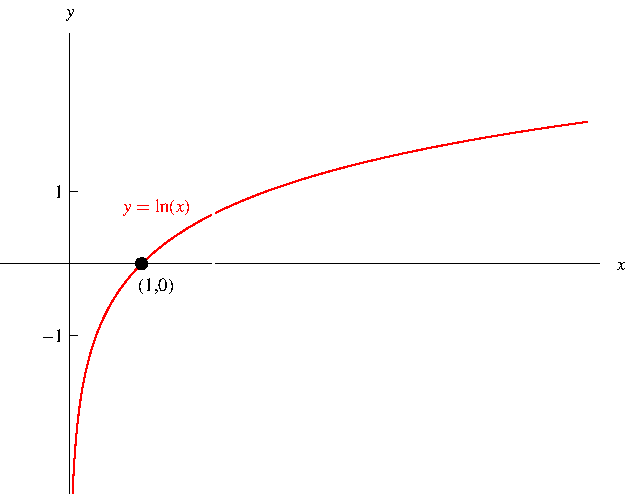
\includegraphics[height=6cm]{logarithms/pictures/07-03-ex8a.pdf}%
%}%
%\only<handout:0| 2>{%
%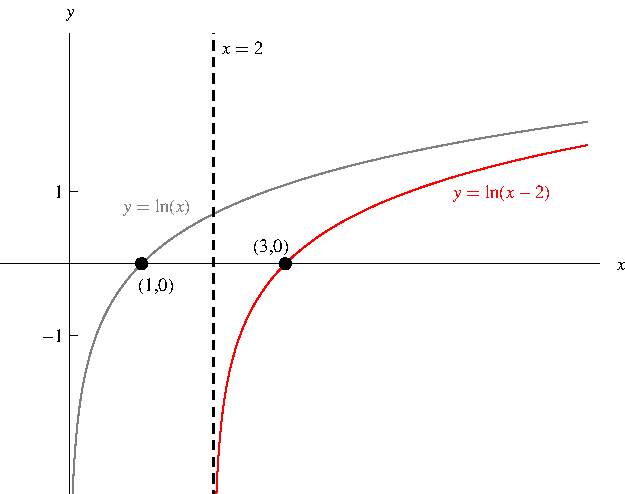
\includegraphics[height=6cm]{logarithms/pictures/07-03-ex8b.pdf}%
%}%
%\only<3->{%
%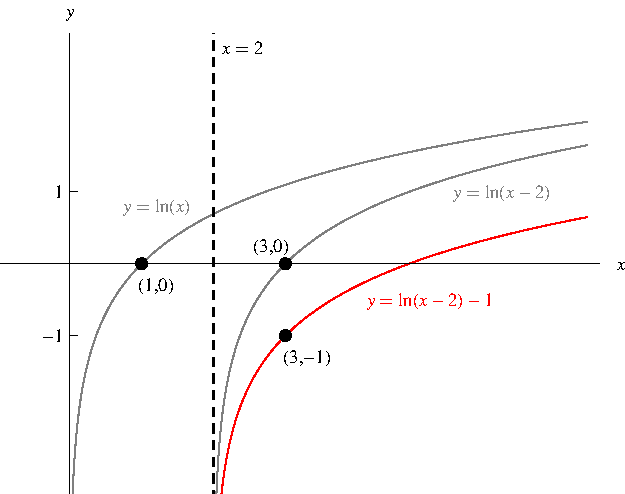
\includegraphics[height=6cm]{logarithms/pictures/07-03-ex8c.pdf}%
%}%
\column{.45\textwidth}
\begin{itemize}
\item<2-> Graph $y=\ln(x)$ assumed given.
\item<3-> $f(x-2)$ shifts graph $2$ units to the right.
\item<4-> $g(x)-1$ shifts graph $1$ unit down.
\end{itemize}
\end{columns}
\end{example}
\end{frame}
% end module natural-logarithm-def-ex8
